%background
\documentclass[../../main/main.tex]{subfiles}


\begin{document}
\title{Background Information}

\chapter{Background}\label{chp:background}
This section aims to provide some background on subjects discussed in this master thesis.  

\section{Formal Methods}
(Primary source for this section is \cite{formalCarnegie})

Formal methods are aimed at improving the reliability and correctness of systems\cite{formalmethodslcarke}.  They are particularly useful in the design phase of systems engineering.  But, they are also employed to varying degrees throughout all aspects of the systems engineering process\footnote{For example, there is notable progress being made in formally verifying c code.  See for example \cite{jvmcmv} and \cite{VARVEL}}.  

Formal methods analysis is a three phase process: (1) formal specification of the system using a modeling language, (2) verification of the specification, and (3) implementation \cite{formalCarnegie}.  Specification consists of describing the system in a mathematical-based modeling language \cite{formalCarnegie}.  Verification entails proving properties of the system, typically using either model checking or theorem proving techniques.  Implementation depends on the type of system (i.e., software, hardware, human-centered system, etc.).

The two most-noted formal methods are model checking and theorem proving.  Model checking involves testing possible states of a system for correctness.  Model checking is touted more as an error checking tool.  It exhausts all possible states (or test states) in search of failures.  But, the absence of failure is not proof of correctness.  Furthermore, for large systems, model checking is resource intensive.  It is subject to the state explosion problem, wherein the number of states of the system grows exponentially with the complexity of the system \cite{stateexplosion}. 

Theorem proving, on the other hand, employs a formal logic to prove properties of the system.  Formal proofs remain true for any test case \cite{formalCarnegie}.  This means that these are proofs of correctness and not just proofs of the absence of failure.  Theorem proving is usually partially or fully automated \cite{wikiformalmethods}.  It often requires specialized knowledge and a sufficient degree of competency in mathematics\footnote{and a good amount of patience, in the author's opinion.}. However, formal theorem proving techniques have been successfully taught to undergraduates\footnote{The PI Professor Shiu-Kai Chin teaches CSBD, which includes theorem proving, to both undergraduates and graduates at Syracuse University.}.  


Model checking and theorem proving often work synergistically.  Both methods offer benefits that the other does not.  As a whole, they improve the reliability of the system's design.   As an example, ElasticSearch successfully applies both methods to its search methodology on distributed systems \cite{elasticsearch}.  

Formal methods are used in some areas of systems engineering more than others.  Some engineers are reluctant to use them because of the additional work and level of expertise required.  However, when correctness is non-negotiable, such as safety and security, formal methods become essential.  Formal methods are predicted to increase in usage as tools become easier to use and engineering curricula increasingly offer formal methods as part of their core\cite{formalCarnegie}.

Specification has its benefits, not only as a precursor to verification, but also as a tool for understanding.  In cases wherein properties of the system are not proved, the act of formally specifying the system adds a degree of rigor to the process. This rigor often brings new insights about the system because it causes the engineer to think more systematically about the system's design.  In addition, the conversion of a field's jargon into a precise specification language also aids in reproducibility and communicability\footnote{The later ideas are not specifically stated in the main cite, but follow logically from the author's perspective.} \cite{formalCarnegie}.  

This master thesis applies formal verification methods, specifically theorem proving, to prove the security properties of a system.  Theorem proving is partially automated using the Higher Order Logic (\glsentryshort{hol}) Interactive Theorem Prover. 

\section{Functional Programming}
(Primary source for this section is \cite{functionalprogramming})

Functional programing is a style of programming that uses functions to define program behavior.  Functional programing is inherently different than procedural or object-oriented programming. These styles of program use procedures or objects and classes to define program behavior.  c  and Pascal are examples of procedural programming languages.  c++ and Java are examples of object-oriented programming languages.  Haskell and ML\footnote{ML is not considered a purely functional.} (meta language) are examples of functional programming languages.  

Functional programming languages are thought to be more pure.  They have fewer side effects than procedural or object-oriented programming.  They produce fewer bugs.  Functional programming languages are thus considered more reliable. This is why theorem provers are typically implemented in functional programming languages.  

This master thesis relies on the Higher Order Logic (HOL) Interactive theorem prover.  HOL is implemented in a functional programming language.  HOL is thought to be very reliable and trustworthy.  Part of that trustworthiness is a function of the meta language in which it is described, namely polyML.

\section{Algebraic Data Types in ML}\label{adt}\label{sec:adtinml}
The primary source for this section is \textit{Introduction to Programming Languages/Algebraic  Data Types} \cite{types}.  This section is helpful in understanding section \ref{sec:aclinhol}.  The reader may skip this section and return to it before reading that section.

The online book \textit{Introduction to Programming Languages/Algebraic  Data Types} describes types as sets.  For example, the boolean type is a set composed of two values "True" and "False".  

An algebraic data type (\glsentryshort{adt}) is a composite data type.  The boolean type is also an \glsentryshort{adt}.  In ML, \glsentryshortpl{adt} are preceded by the \texttt{datatype} keyword.  The boolean data type would be defined as:

A note on type constructors: in ML\footnote{Standard ML according to the author \cite{constructor}.} a type constructors should be thought of as a function that takes a type as its parameter and returns a type.  In the declaration \texttt{Node of 'a tree * 'a * 'a tree}. \texttt{Node} behaves like a function which returns something of type \texttt{'a tree} \cite{constructor}.  

\begin{figure}[h]
\centering
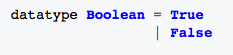
\includegraphics[width=0.4\textwidth]{../figures/booladt}
\caption{\label{booladt} An implementation of the boolean datatype in ML.  Image from \textit{Introduction to Programming Languages/Algebraic Data Types} \cite{types} }.  
\end{figure}

The boolean datatype can be thought of as the union of the the two singleton sets "True" and "False".  The \textbar symbol denotes union in this case.  

An example of a more complicated datatype is the tree datatype defined below.

\begin{figure}[h]
\centering
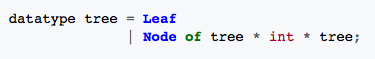
\includegraphics[width=0.6\textwidth]{../figures/tree}
\caption{\label{tree} An implementation of a tree datatype in ML.  Image from \textit{Introduction to Programming Languages/Algebraic Data Types} \cite{types} }.  
\end{figure}

The first element of the tree datatype is "Leaf".  The second element is a "Node".  The node has three components: tree, int, and another tree.  The "of" keyword in ML indicates that what follows is a type.  Thus, this is a "Node" \textbf{of} type tree * int * tree.  The * symbol represents the cartesian product.  The easiest way to think of this particular example in ML is that the "Node" type is a three-tuple consisting of (tree, int, tree).

\glsentryshortpl{adt} exhibit the property of pattern matching.  This is typical of functional programming languages.  For example, consider the datatype weekday shown below.

\begin{figure}[h]
\centering
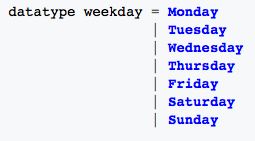
\includegraphics[width=0.5\textwidth]{../figures/weekday}
\caption{\label{weekday} An implementation of the weekday datatype in ML.  Image from \textit{Introduction to Programming Languages/Algebraic Data Types} \cite{types} }.  
\end{figure}

With pattern matching, it is possible to define a function is_weekend which returns "True" if it is a weekend and "False" otherwise.  Consider the following definition for a function that takes one argument (or parameter) of type "weekday."


\begin{figure}[h]
\centering
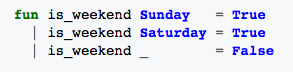
\includegraphics[width=0.5\textwidth]{../figures/isweekend}
\caption{\label{isweekend} An implementation of the function is_weekend in ML.  Image from \textit{Introduction to Programming Languages/Algebraic Data Types} \cite{types} }.  
\end{figure}


The keyword "fun" must precede any function definition in ML. Next, is the name of the function, in this case "is_weekend".  The next word "Sunday" is an element of the datatype "weekday."  When ML evaluates the "is_weekend" function, it will check the argument.  If the argument is "Sunday" then ML will return "True", otherwise it will check the next line.  If the argument equals "Saturday" ML will return "True", otherwise it will check the next line.  The next line contains the underscore character.  In ML, this is similar to the wildcard * character in Unix.  In this case, the underscore character tells ML to return "False" for any argument.  The novelty of pattern matching is that function evaluation proceeds in order, allowing for an easy and clean way to define an if-then-else evaluation.

A second property of \glsentryshortpl{adt} is parameterization.  Consider a more general definition of the tree datatype shown below.

\begin{figure}[h]
\centering
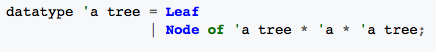
\includegraphics[width=0.6\textwidth]{../figures/treeparam}
\caption{\label{treeparam} A parameterized implementation of a tree datatype in ML.  Image from \textit{Introduction to Programming Languages/Algebraic Data Types} \cite{types} }.  
\end{figure}

In this definition, the datatype definition is preceded by the type variable \texttt{'a}.  To declare something of type \texttt{'a Tree}, the \texttt{'a} is instantiated.  For example, \texttt{int tree}, produces the same tree is the original definition.  

\texttt{'a} is called a polymorphic type or type variable.  A type variable is just a place holder for some other type or type variable.  Type variables are always preceded with a forward tick mark (apostrophe) in ML.


\section{Higher Order Logic (HOL) Interactive Theorem Prover}
The Higher Order Logic (HOL) Interactive theorem prover is a proof assistant.  HOL has proved to be a very reliable theorem proving system.  It is widely trusted in the interactive theorem proving community.

At its core, HOL implements a small set of axioms and a formal logic.  All inferences and theorems must be derived from this small set of axioms using the formal logic.  Reasoning logically with a small set of axioms contributes to the trustworthiness of the system.  The user only has to trust the small set of axioms and the logic (in addition to HOL's implementation).  Beyond the competence of the programmer, it is said that if it can't be proved in HOL then it can be proved.  

HOL is a strongly-typed system.  This means that data has a predefined type.  As in all functional programming languages, the type of these data can not change.  This adds to the reliability of HOL by preventing side-effects. HOL has several built-in data types.  But, the user can also define her own data type.   In addition to datatypes, the user can define her own set of axioms and definitions.  

With user-defined types, axioms, and definitions, the user can describe a system in HOL and then use HOL's formal logic to prove properties of this system.  This is the basis for theorem proving in formal methods.

The version of HOL used for this master thesis is HOL4.  HOL4 is free software that is BSD licensed \cite{BSDlicenses}.  Download instructions can be found at the HOL website hol-theorem-prover.og \cite{HOL}.According to Wikipedia, HOL4 is descended from HOL88.  The HOL88 project is Mike Gordon's effort..  HOL4 is implemented in polyML which is an implementation of Standard ML \cite{HOLwiki}.

\section{Other Interactive Theorem Provers}
It should be noted that HOL is not unique. There are other interactive theorem provers on the market. Each has its own niche and dedicated user base.  Choice of theorem prover is typically guided by personal preference and familiarity. The later follows from the somewhat steep learning curve for theorem provers. 

For example, Isabelle/HOL\footnote{The author is interested in implementing more of the ACL and secure state machines in Isabelle/HOL.} is another popular interactive theorem prover.  The access-control logic (\glsentryshort{acl})has been partially implemented in Isabelle/HOL by Scott Constable, a PhD student in the College of Engineering and Computer Science and Syracuse University.  

\section{How to Compile The Included Files}
All the files necessary to compile the theories discussed in this mater thesis are included.  A diagram of the folder structure is included in the appendix \ref{foldermap}.  To compile the theories and the LaTeX files go to the folder titled MasterThesis.  Open up a terminal.  Type \emph{make} and then hit enter.  Note that to compile the theories HOL and LaTeX must be first be installed.  


\end{document}